%%%%%%%%%%%%%%%%%%%%%%%%%%%%%%%%%%%%%%%%%%%%%%%%%%%%%%%%%%%%%%%
\chapter{基于概率逻辑推理的问答系统的设计和实现}{Implementaion: A Question Answering System Based on Probabilistic Logic Reasoning}
\label{chap:dialogue}
%%%%%%%%%%%%%%%%%%%%%%%%%%%%%%%%%%%%%%%%%%%%%%%%%%%%%%%%%%%%%%%


本文的智能对话系统的预期目标主要是实现面向游戏角色和人型机器人的对话系统,但同样的研究思路也完全适用于基于文本的对话系统,例如智能对话搜索接口。我们分阶段来实现这样的目标,首先以一些相对小二简单的智能对话系统为起点,通过不断改进和完善,以及结合系统本身的自学习和人只能里,最终实现一个在一定程度上接近人类智能水平的对话系统。本章就根据第\ref{chap:dialogueModel}章中提出的智能对话系统CogDial的概念模型,并结合第\ref{chap:comprehension}章的自然语言理解技术以及第\ref{chap:generation}章自然语言生成技术的研究成果,设计并实现了几个基于概率逻辑推理的问答系统。除此之外,本章还结合我们研究中的发现和遇到的难题对深层语义解析的挑战进行了讨论,也给未来的研究提供了一个明确的方向。

需要说明的是,目前该系统只能处理英文对话,所以接下来介绍系统的设计和实现时所举的对话例子基本是按照英文习惯,可能不太适合中文的语言习惯,但是该系统所采用的技术和理论基础都是完全适合中文的。


%%%%%%%%%%%%%%%%%%%%%%%%%%%%%%%%%%%%%%%%%%%%%%%%%%%%%%%%%%%%%%%
\section{基于超图模糊匹配的问答系统}{Question-Answering Via Hypergraph Fuzzy Matching}
%%%%%%%%%%%%%%%%%%%%%%%%%%%%%%%%%%%%%%%%%%%%%%%%%%%%%%%%%%%%%%%

为了实现我们的智能对话系统的框架以及设计思路,我们构建了一个基于超图模糊匹配的问答系统的原型,该问答系统使用前文提到的自然语言理解技术将自然语言转换成以超图表示的语义逻辑形式,利用基于超图匹配的动态编程算法,从而在问答语料库中找到最适合问题的答案来响应用户查询。

本节首先讨论该问答系统框架中使用的超图匹配算法,然后再讨论基于超图模糊匹配的问答系统的设计和实现。

\subsection{基于超图的模式匹配器}{The Hypergraph Pattern Matcher}

基于超图的模式匹配器是一个查询引擎或变数配对者,主要功用是在我们的超图知识库Atomspace中寻找特定的模式,或是一些Atom相关排列或“模板“。在轮入一个等定的Atom排列(即一个超图)后,模式匹配器会从Atomspace中寻找所有合乎条件的超图。同时一些“空白位置“,即“变数“在一个超图的位置,亦可存在于该输入的超图当中,而模式匹配器则会“填补“这些“空白位置“。例如:“John threw a \_\_\_\_).“亦可以被判断为“John threw a ball.“,前提是在查询前该句子要存在于Atomspace里,而在这个例子中“ball“就是被配对的一个答案。输入的超图中可以在不同的地方拥有多过一个的“空白位置“,同时亦可以有多过一个的答案。在这过程中,BindLink提供了一个便利的API去达到这目的,接下来会有更多的技术层面说明。

模式匹配器是一个变数配对者,是在传统计算机科学中“统一“的概念,因为这是它的功能之一。它同时亦是一个查询引擎,因为这个变数配对过程某情度上是等同于用SQL在关联数据库中进行查询。其中主要的分别在于在我们这里的概念是以超图的形式表示,所以它亦可以被形容为一个超图查询语言HQL(Hypergraph Query Language)。但这些都只是以不同的名称去表示同一个程序。

这个模式匹配器是结构精密应用的一个重要组件,同时也是建立逻辑推理系统中前向和后向链接推理的一个重要基础。它拥有C++和Scheme的接口以供不同的应用。

模式匹配器由数个不同的组件连接在一起,组成一个基础前向链接或超图重写的工具。在其核心是一个能比较和配对不同超图以及其变数的组件,而这个组件跟另一个“找寻器“一同使用便能寻找整个Atomspace中的合乎条件的超图。最后一个组件是一个“编写器“,主要功用是当有一个配对成功产生后建立一个或以上在ImplicationLink后半部列明的超图。

这个模式匹配器接受有指定“规则“的BindLinks,再把这些“规则“应用到Atomspace里。每一个“规则“是一个ImplicationLink,以“if P then Q“的形式表达,当中P和Q分别代表不同的超图。如果P被实现了,那么便能得到Q。Q可以是任何种类的超图,但如果Q是一个ExecutionLink,这便意味著当P被实现了,系统便将会实行其他程序,这在整体来说可以是一个十分强大的功能,因为在一般情况下很多程序都可以以ExecutionLink来执行。

模式匹配器不会更改任何超图中的真值(Truth Value)或关注值(Attention Value),有需要时使用者亦可以自行编写和执行相关的程序。

在默认的回调函数中模式匹配器会搜索整个Atomspace,因此亦有需要编写特定的回调函数以限制其搜索范围,例如只寻找和接受拥有某程度短期重要性的Atom,以只获取相对重要的资讯。

以下是一个使用模式匹配器的示例:

\begin{verbatim}
(define find-animals
  (BindLink
    ;; The variable to be bound
    (VariableNode "$var")
    (ImplicationLink
      ;; The pattern to be searched for
      (InheritanceLink
         (VariableNode "$var")
         (ConceptNode "animal")
      )

      ;; The value to be returned.
      (VariableNode "$var")
    )
  )
)
 \end{verbatim}

执行时,只需在我们系统的Scheme终端输入以下指令便能执行以上的模式匹配器并找出在Atomspace中所有继承“animal“的概念:

\begin{verbatim}
(cog-bind find-animals)
\end{verbatim}

\subsection{基于超图模糊匹配的问答系统}

本小节我们将阐述这个基于超图的模糊匹配的启发式的问答系统的设计思路和实现方法,该系统主要针对信息查询。其基本算法可简单概括如下:给定一个查询Q,通过我们的自然语言理解流水线将其转换成Atomspace里的超图形式,然后在知识库Atomspace 里找出与其相似的表示陈述句的超图。这里我们做了一个合理的猜测,认为这些相似的超图中的其中一个包含了Q的答案。

如果给定一个很大的超图H,在H的所有子图中找到与目标超图Q部分匹配的子超图是一个非常困难的计算问题。我们使用了启发式在一定程度上解决了计算难度,虽然这不能保证找到问题的正确答案,但实验发现该方法通常能找到一个很好的答案。我们的启发式涉及下面两个阶段:

\begin{itemize}
\item {\bf 第一阶段:}使用一个基于超图的模糊匹配器Pattern Matcher,搜索能正确回答查询Q的答案。在此搜索过程中,保存所有与查询Q近似匹配的子超图。
\item {\bf 第二阶段:}对第一阶段中的所有部分匹配的子超图,使用基于超图匹配的动态规划来计算它们的匹配程度,然后根据匹配程度进行排序。
\end{itemize}
基于超图匹配的动态规划是对 \cite{Zass2008}中的算法一个新的改进。正如基于动态规划的字符串匹配,获得高性能的一个重要因素是从源到目标的路径转换过程中合理地分配具体的操作成本。我们对此使用的启发式如下:修改(可以是添加、删除或替换)一个稀有词对应的节点比修改一个常用词对应的节点的成本高;修改一个稀有词节点对应的链比修改一个常用词节点对应的链的成本高。这里的“稀有程度”通过词频或者该词所关联的WordNode, ConceptNode或者PredicateNode的真值来衡量。

假设所需的查询是“Who bought a glockenspiel at the store?”(谁在商店买了一个钟琴?),那么如果将“glockenspiel”替换成其他词的时候,那其成本就比将“store”替换成其他词要高,因为“glockenspiel”比“store”更稀有。因此“Bob bought a glockenspiel with his friend.”(Bob和他朋友一起买了钟琴。)和查询的匹配程度要高于“Jim bought a thimble at the store.”(Jim在商店买了一个针箍。)。

这种基于频率的启发式相当于实例化OpenCog里经常使用的一个一般原则:信息含量往往通过概率化的惊讶度来衡量。发现句子里的“glockenspiel”比发现“store”的惊讶度更高,因此,我们断定,在此查询中,“glockenspiel”含有的信息量更大,所以当修改“glockenspiel”的时候会被分配很高的成分,因为做这样的修改就相当于删除了查询中的较多的信息。这样的信息论原则也给OpenCog中的Pattern Mining\cite{ONeill2012} 奠定了基础, Pattern Mining在OpenCog的动机机制中充当了重要的角色,可以用来满足我们前面提到的OpenPsi里的“新颖性”(Novelty)的目标需求。一个更智能更复杂的匹配方法可以根据总体惊讶值来惩罚修改序列,但目前的做法依然是只针对查询的各个部分的惊讶度单独作为指标,待系统逐步改善后,会考虑实现更复杂的匹配算法。
为了简化操作,在做查询匹配的过程中,我们忽略了表示查询的超图中很多不重要的Atoms,仅表明语义关系的核心部分用于匹配。对于例句“Who bought a glockenspiel at the store?”,仅有下面这些Atoms参与超图匹配:

 {\tt\begin{tiny}\begin{lstlisting}
((ReferenceLink
   (InterpretationNode "sentence@ae4_parse_0_interpretation_$X")
   (SetLink
      (ImplicationLink (stv 0.99000001 0.99000001)
         (PredicateNode "bought@530" (stv 0.001 0.99000001))
         (PredicateNode "buy" (ptv 0.001 0.99000001 1))
      )
      (InheritanceLink (stv 0.99000001 0.99000001)
         (ConceptNode "glockenspiel@bf4" (stv 0.001 0.99000001))
         (ConceptNode "glockenspiel" (ptv 0.001 0.99000001 1))
      )
      (InheritanceLink (stv 0.99000001 0.99000001)
         (ConceptNode "store@ae4" (stv 0.001 0.99000001))
         (ConceptNode "store" (ptv 0.001 0.99000001 1))
      )
      (EvaluationLink (stv 0.99000001 0.99000001)
         (PredicateNode "bought@530" (stv 0.001 0.99000001))
         (ListLink (stv 0.99000001 0.99000001)
            (VariableNode "$rIr" (stv 0.001 0.99000001))
            (ConceptNode "glockenspiel@bf4" (stv 0.001 0.99000001))
            (ConceptNode "store@ae4" (stv 0.001 0.99000001))
         )
      )
      (InheritanceLink (stv 0.99000001 0.99000001)
         (ConceptNode "at@d68" (stv 0.001 0.99000001))
         (ConceptNode "at" (ptv 0.001 0.99000001 1))
      )
      (InheritanceLink (stv 0.99000001 0.99000001)
         (SatisfyingSetLink (stv 0.99000001 0.99000001)
            (PredicateNode "bought@530" (stv 0.001 0.99000001))
         )
         (ConceptNode "at@d68" (stv 0.001 0.99000001))
      )
      (InheritanceLink (stv 0.99000001 0.99000001)
         (PredicateNode "bought@530" (stv 0.001 0.99000001))
         (ConceptNode "past" (stv 0.001 0.99000001))
      )
      (EvaluationLink (stv 0.99000001 0.99000001)
         (PredicateNode "definite" (stv 0.001 0.99000001))
         (ListLink (stv 0.99000001 0.99000001)
            (ConceptNode "store@ae4" (stv 0.001 0.99000001))
         )
      )
      (ImplicationLink (stv 0.99000001 0.99000001)
         (PredicateNode "at@d68" (stv 0.001 0.99000001))
         (PredicateNode "at" (ptv 0.001 0.99000001 1))
      )
      (EvaluationLink (stv 0.99000001 0.99000001)
         (PredicateNode "at@d68" (stv 0.001 0.99000001))
         (ListLink (stv 0.99000001 0.99000001)
            (ConceptNode "store@ae4" (stv 0.001 0.99000001))
         )
      )
      (InheritanceLink (stv 0.001 0.99000001)
         (InterpretationNode "sentence@ae4_parse_0_interpretation_$X")
         (ConceptNode "InterrogativeSpeechAct" (stv 0.001 0.99000001))
      )
   )
)
)

\end{lstlisting}\end{tiny}}

类似地,我们使用简化过的表示“Bob mauled a glockenspiel with his friend.”的超图:

 {\tt\begin{tiny}\begin{lstlisting}
((ReferenceLink
   (InterpretationNode "sentence@477_parse_0_interpretation_$X")
   (SetLink
      (ImplicationLink (stv 0.99000001 0.99000001)
         (PredicateNode "mauled@1a0" (stv 0.001 0.99000001))
         (PredicateNode "maul" (ptv 0.001 0.99000001 1))
      )
      (InheritanceLink (stv 0.99000001 0.99000001)
         (ConceptNode "Bob@1c3" (stv 0.001 0.99000001))
         (ConceptNode "Bob" (ptv 0.001 0.99000001 1))
      )
      (InheritanceLink (stv 0.99000001 0.99000001)
         (ConceptNode "glockenspiel@b12" (stv 0.001 0.99000001))
         (ConceptNode "glockenspiel" (ptv 0.001 0.99000001 1))
      )
      (InheritanceLink (stv 0.99000001 0.99000001)
         (ConceptNode "friend@e78" (stv 0.001 0.99000001))
         (ConceptNode "friend" (ptv 0.001 0.99000001 1))
      )
      (EvaluationLink (stv 0.99000001 0.99000001)
         (PredicateNode "mauled@1a0" (stv 0.001 0.99000001))
         (ListLink (stv 0.99000001 0.99000001)
            (ConceptNode "Bob@1c3" (stv 0.001 0.99000001))
            (ConceptNode "glockenspiel@b12" (stv 0.001 0.99000001))
            (ConceptNode "friend@e78" (stv 0.001 0.99000001))
         )
      )
      (InheritanceLink (stv 0.99000001 0.99000001)
         (ConceptNode "with@8ef" (stv 0.001 0.99000001))
         (ConceptNode "with" (ptv 0.001 0.99000001 1))
      )
      (InheritanceLink (stv 0.99000001 0.99000001)
         (SatisfyingSetLink (stv 0.99000001 0.99000001)
            (PredicateNode "mauled@1a0" (stv 0.001 0.99000001))
         )
         (ConceptNode "with@8ef" (stv 0.001 0.99000001))
      )
      (InheritanceLink (stv 0.99000001 0.99000001)
         (PredicateNode "mauled@1a0" (stv 0.001 0.99000001))
         (ConceptNode "past" (stv 0.001 0.99000001))
      )
      (InheritanceLink (stv 0.001 0.99000001)
         (InterpretationNode "sentence@477_parse_0_interpretation_$X")
         (ConceptNode "DeclarativeSpeechAct" (stv 0.001 0.99000001))
      )
      (EvaluationLink (stv 0.99000001 0.99000001)
         (PredicateNode "definite" (stv 0.001 0.99000001))
         (ListLink (stv 0.99000001 0.99000001)
            (ConceptNode "friend@e78" (stv 0.001 0.99000001))
         )
      )
      (InheritanceLink (stv 0.99000001 0.99000001)
         (ConceptNode "his@301" (stv 0.001 0.99000001))
         (ConceptNode "his" (ptv 0.001 0.99000001 1))
      )
      (EvaluationLink (stv 0.99000001 0.99000001)
         (PredicateNode "possession" (stv 0.001 0.99000001))
         (ListLink (stv 0.99000001 0.99000001)
            (ConceptNode "friend@e78" (stv 0.001 0.99000001))
            (ConceptNode "his@301" (stv 0.001 0.99000001))
         )
      )
      (ImplicationLink (stv 0.99000001 0.99000001)
         (PredicateNode "with@8ef" (stv 0.001 0.99000001))
         (PredicateNode "with" (ptv 0.001 0.99000001 1))
      )
      (EvaluationLink (stv 0.99000001 0.99000001)
         (PredicateNode "with@8ef" (stv 0.001 0.99000001))
         (ListLink (stv 0.99000001 0.99000001)
            (ConceptNode "friend@e78" (stv 0.001 0.99000001))
         )
      )
      (InheritanceLink (stv 0.99000001 0.99000001)
         (SpecificEntityNode "Bob@1c3" (stv 0.001 0.99000001))
         (ConceptNode "male" (stv 0.001 0.99000001))
      )
      (InheritanceLink (stv 0.99000001 0.99000001)
         (SpecificEntityNode "Bob@1c3" (stv 0.001 0.99000001))
         (ConceptNode "Bob" (ptv 0.001 0.99000001 1))
      )
      (EvaluationLink (stv 0.99000001 0.99000001)
         (PredicateNode "definite" (stv 0.001 0.99000001))
         (ListLink (stv 0.99000001 0.99000001)
            (ConceptNode "Bob@1c3" (stv 0.001 0.99000001))
         )
      )
   )
)
)

\end{lstlisting}\end{tiny}}

和表示”Jim bought a thimble at the store.”的超图

 {\tt\begin{tiny}\begin{lstlisting}
((ReferenceLink
   (InterpretationNode "sentence@d92_parse_0_interpretation_$X")
   (SetLink
      (ImplicationLink (stv 0.99000001 0.99000001)
         (PredicateNode "bought@7e4" (stv 0.001 0.99000001))
         (PredicateNode "buy" (ptv 0.001 0.99000001 1))
      )
      (InheritanceLink (stv 0.99000001 0.99000001)
         (ConceptNode "Jill@bc3" (stv 0.001 0.99000001))
         (ConceptNode "Jill" (ptv 0.001 0.99000001 1))
      )
      (InheritanceLink (stv 0.99000001 0.99000001)
         (ConceptNode "thimble@8a3" (stv 0.001 0.99000001))
         (ConceptNode "thimble" (ptv 0.001 0.99000001 1))
      )
      (InheritanceLink (stv 0.99000001 0.99000001)
         (ConceptNode "store@ef6" (stv 0.001 0.99000001))
         (ConceptNode "store" (ptv 0.001 0.99000001 1))
      )
      (EvaluationLink (stv 0.99000001 0.99000001)
         (PredicateNode "bought@7e4" (stv 0.001 0.99000001))
         (ListLink (stv 0.99000001 0.99000001)
            (ConceptNode "Jill@bc3" (stv 0.001 0.99000001))
            (ConceptNode "thimble@8a3" (stv 0.001 0.99000001))
            (ConceptNode "store@ef6" (stv 0.001 0.99000001))
         )
      )
      (InheritanceLink (stv 0.99000001 0.99000001)
         (ConceptNode "at@50d" (stv 0.001 0.99000001))
         (ConceptNode "at" (ptv 0.001 0.99000001 1))
      )
      (InheritanceLink (stv 0.99000001 0.99000001)
         (SatisfyingSetLink (stv 0.99000001 0.99000001)
            (PredicateNode "bought@7e4" (stv 0.001 0.99000001))
         )
         (ConceptNode "at@50d" (stv 0.001 0.99000001))
      )
      (InheritanceLink (stv 0.99000001 0.99000001)
         (PredicateNode "bought@7e4" (stv 0.001 0.99000001))
         (ConceptNode "past" (stv 0.001 0.99000001))
      )
      (InheritanceLink (stv 0.001 0.99000001)
         (InterpretationNode "sentence@d92_parse_0_interpretation_$X")
         (ConceptNode "DeclarativeSpeechAct" (stv 0.001 0.99000001))
      )
      (EvaluationLink (stv 0.99000001 0.99000001)
         (PredicateNode "definite" (stv 0.001 0.99000001))
         (ListLink (stv 0.99000001 0.99000001)
            (ConceptNode "store@ef6" (stv 0.001 0.99000001))
         )
      )
      (ImplicationLink (stv 0.99000001 0.99000001)
         (PredicateNode "at@50d" (stv 0.001 0.99000001))
         (PredicateNode "at" (ptv 0.001 0.99000001 1))
      )
      (EvaluationLink (stv 0.99000001 0.99000001)
         (PredicateNode "at@50d" (stv 0.001 0.99000001))
         (ListLink (stv 0.99000001 0.99000001)
            (ConceptNode "store@ef6" (stv 0.001 0.99000001))
         )
      )
      (InheritanceLink (stv 0.99000001 0.99000001)
         (SpecificEntityNode "Jill@bc3" (stv 0.001 0.99000001))
         (ConceptNode "female" (stv 0.001 0.99000001))
      )
      (InheritanceLink (stv 0.99000001 0.99000001)
         (SpecificEntityNode "Jill@bc3" (stv 0.001 0.99000001))
         (ConceptNode "Jill" (ptv 0.001 0.99000001 1))
      )
      (EvaluationLink (stv 0.99000001 0.99000001)
         (PredicateNode "definite" (stv 0.001 0.99000001))
         (ListLink (stv 0.99000001 0.99000001)
            (ConceptNode "Jill@bc3" (stv 0.001 0.99000001))
         )
      )
   )
)
)

\end{lstlisting}\end{tiny}}

我们的下一步研究会将逻辑推理也加入成本计算的过程,从而进一步改进上述针对查询处理的超图匹配。假如知识库中代表下面这个句子的超图表示“Jim bought a musical instrument at the store.”(Jim 在商店买了一个乐器。),那么如果该查询系统能做出以下推理:

\begin{verbatim}
InheritanceLink
	ConceptNode "glockenspiel"
	ConceptNode "musical instrument"
\end{verbatim}

得到“钟琴”是一种“乐器”,那么会对“钟琴”改为“乐器”的修改操作赋值一个较低的成本值。基于这样的简单推理,系统会认为“Jim bought a musical instrument at the store.”(Jim在商店买了一个乐器)比“ Jim bought a power tool at the store.” (Jim在商店买了一个电源工具)更符合上述查询。

%%%%%%%%%%%%%%%%%%%%%%%%%%%%%%%%%%%%%%%%%%%%%%%%%%%%%%%%%%%%%%%
\section{基于后向链接推理的问答系统}{Question-Answering via Backward Chaining Reasoning}
\label{sec:backward}
%%%%%%%%%%%%%%%%%%%%%%%%%%%%%%%%%%%%%%%%%%%%%%%%%%%%%%%%%%%%%%%

上一节中介绍的基于超图匹配的问答虽然能回答不少的查询,但是随着知识库Atomspace的不断变大,搜索匹配的工作会变得越来越复杂,也越来越耗时。而且基于超图匹配的方法只是一个粗糙的启发式搜索过程,不适用于这些情况:对查询时间要求高、知识库数据不足或者在知识库中的答案需要经过一定推理才能找到等。例如,该方法无法将查询“Who bought a glockenspiel?”(谁买了钟琴?)从下面的句子中找到近似匹配,但是这些句子都在一定程度上暗示了此查询的答案。

\begin{itemize}
\item Bob brought his new instrument home from the mall and played it for his kids.(Bob从商场带了新乐器回家,并为他的孩子们演奏了几曲。)
\item Ling-ling's house is like a museum of obscure musical instruments.(玲玲的家像一个稀有乐器博物馆)
\item Jack always buys whatever he sees in a magazine. ... On the flight back from Guilin, there was nothing for Jack to read but a catalog of weird musical instruments.(Jack总爱买任何他在杂志上看到的东西。在从桂林回来的飞机上,只给Jack提供了一本稀奇乐器相关的杂志)
\end{itemize}

从另一方面来说,经过在适当的知识库上推理,也不难从上面的句子中找出适合此查询的答案。例如,如果想从第二个句子“Ling-ling's house is like a museum of obscure musical instruments.”中找出符合查询的答案,我们可通过如下推理得到:

\begin{verbatim}
Ling-ling's house is like a museum of obscure musical instruments
(玲玲的家像一个稀有乐器博物馆。)

The glockenspiel is obscure, and the glockenspiel is a musical instrument
(钟琴很稀有,而且钟琴是一种乐器。)

A museum of entities of type X, contains many instances of X
(有关X的博物馆,含有很多X的实例。)

If X is in Y's house, then often Y has bought X
(如果Y的家中有X,那么通常Y买了X。)

|-

It is non-trivially probable that Ling-ling has bought a glockenspiel
(玲玲很有可能买了一个钟琴。)
\end{verbatim}

在Atomspace中,这样的定性推理可以通过不同很多方式进行。下面我们将解释其中一种方式的推理过程。推理的前提可表示如下:

\begin{verbatim}

Ling-ling's house is like a museum of obscure musical instruments:
(玲玲的家像一个稀有乐器博物馆。)

InheritanceLink
	ConceptNode "house@123"
	ConceptNode "house"
	
EvaluationLink
	PredicateNode "own"
	ConceptNode "Ling-ling"
	ConceptNode "house@123"

SimilarityLink
	ConceptNode "house@123"
	ConceptNode "museum@552"
	
InheritanceLink
	ConceptNode "museum@552"
	ConceptNode "museum"

EvaluationLink
	PredicateNode "of"
	ConceptNode "museum@552"
	ConceptNode "instruments@12d"
	
InheritanceLink
	ConceptNode "instruments@12d"
	ConceptNode "obscure"
	
InheritanceLink
	ConceptNode "instruments@12d"
	ConceptNode "musical"	
	
InheritanceLink
	ConceptNode "instrument@12d"
	ConceptNode "instrument"	
	
The glockenspiel is obscure, and the glockenspiel is a musical instrument:
(钟琴很稀有,而且钟琴是一种乐器。)

InheritanceLink
	ConceptNode "glockenspiel"
	ConceptNode "obscure"
	
InheritanceLink
	ConceptNode "glockenspiel"
	ConceptNode "instrument@1c5"
	
InheritanceLink
	ConceptNode "instrument@1c5"
	ConceptNode "musical"
	
InheritanceLink
	ConceptNode "instrument@1c5"
	ConceptNode "obscure"	
	
InheritanceLink
	ConceptNode "instrument@1c5"
	ConceptNode "instrument"		

A museum of entities of type X, contains many instances of X:
(有关X的博物馆,含有很多X的实例。)

ImplicationLink  <.95,.99>
	ANDLink
		InheritanceLink
			$X
			ConceptNode "museum"
		EvaluationLink
			PredicateNode "of"
			$X
			$Z
	EvaluationLink
		PredicateNode "many"
		SatisfyingSetLink
			ANDLink
				InheritanceLink
					$A
					$Z
				EvaluationLink
					PredicateNode "in"
					$A
					X

If X is in Y's house, then often Y has bought X:
(如果Y的家中有X,那么通常Y买了X。)

ImplicationLink <.8,.9>
	ANDLink
		EvaluationLink
			PredicateNode "in"
			ListLink
				$X
				$Z
		InheritanceLink
			$Z
			ConceptNode "house"
		EvaluationLink
			PredicateNode "own"
			ListLink
				$Y
				$Z
	EvaluationLink
		PredicateNode "buy"
		ListLink
			$Y
			$X

\end{verbatim}

根据上面的推理前提,PLN可以推理得到下面的结论:

\begin{verbatim}
EvaluationLink <s,c>
	PredicateNode "buy"
	ConceptNode "Ling-ling"
	ConceptNode "glockenspiel"
\end{verbatim}

真值$<s,c>$的大小不仅取决于推理过程中的使用到的推理规则的具体参数,还取决于节点本身的概率大小( “glockenspiel”节点的概率值用于表示钟琴在这世界上有多常见,这有助于估算钟琴是稀有乐器的概率)。因此,即使推理的前提给出很高的强度和置信度的真值如$<1,.95>$,推断得出的结论的真值也可能很低如$<.05,.6>$。不过由于推理的不确定性,得到的这样的低真值结论也是合理的。
上面例子给出的前提是简化过的,比如,没有给出这样的事实:“博物馆通常有稀有的东西”,可表示如下:

\begin{verbatim}
ImplicationLink <.3,.8>
	ANDLink
		InheritanceLink
			$X
			ConceptNode "museum"
		EvaluationLink
			PredicateNode "in"
			$X
			$Z
	InheritanceLink
		$Z
		ConceptNode "obscure"
\end{verbatim}

对该事实的考虑将在一定程度上增加结论的强度。
总的来说,在推理链中不同阶段选择不同的前提,导致可以通过很多不同推理路径得到一个推理结论。每一条推理规则的执行是精确的,但对于选择哪条推理链则是一个非常模糊的问题,需要知识库Atomspace中的具体知识来指导。目前我们的逻辑系统PLN能完成上面的推理,但使用自然语言输入来进行这样的推理还存在一些问题。


%%%%%%%%%%%%%%%%%%%%%%%%%%%%%%%%%%%%%%%%%%%%%%%%%%%%%%%%%%%%%%%
\section{一个综合的问答规划器}{A Composite Question-Answering Schema}
%%%%%%%%%%%%%%%%%%%%%%%%%%%%%%%%%%%%%%%%%%%%%%%%%%%%%%%%%%%%%%%

综合上述对问答规划的讨论,我们还针对信息查找问题设计并实现了一个合理的综合问答规划器,设计思路可参考图\ref{fig:QA-schema}

\begin{figure}[htb]
\centering
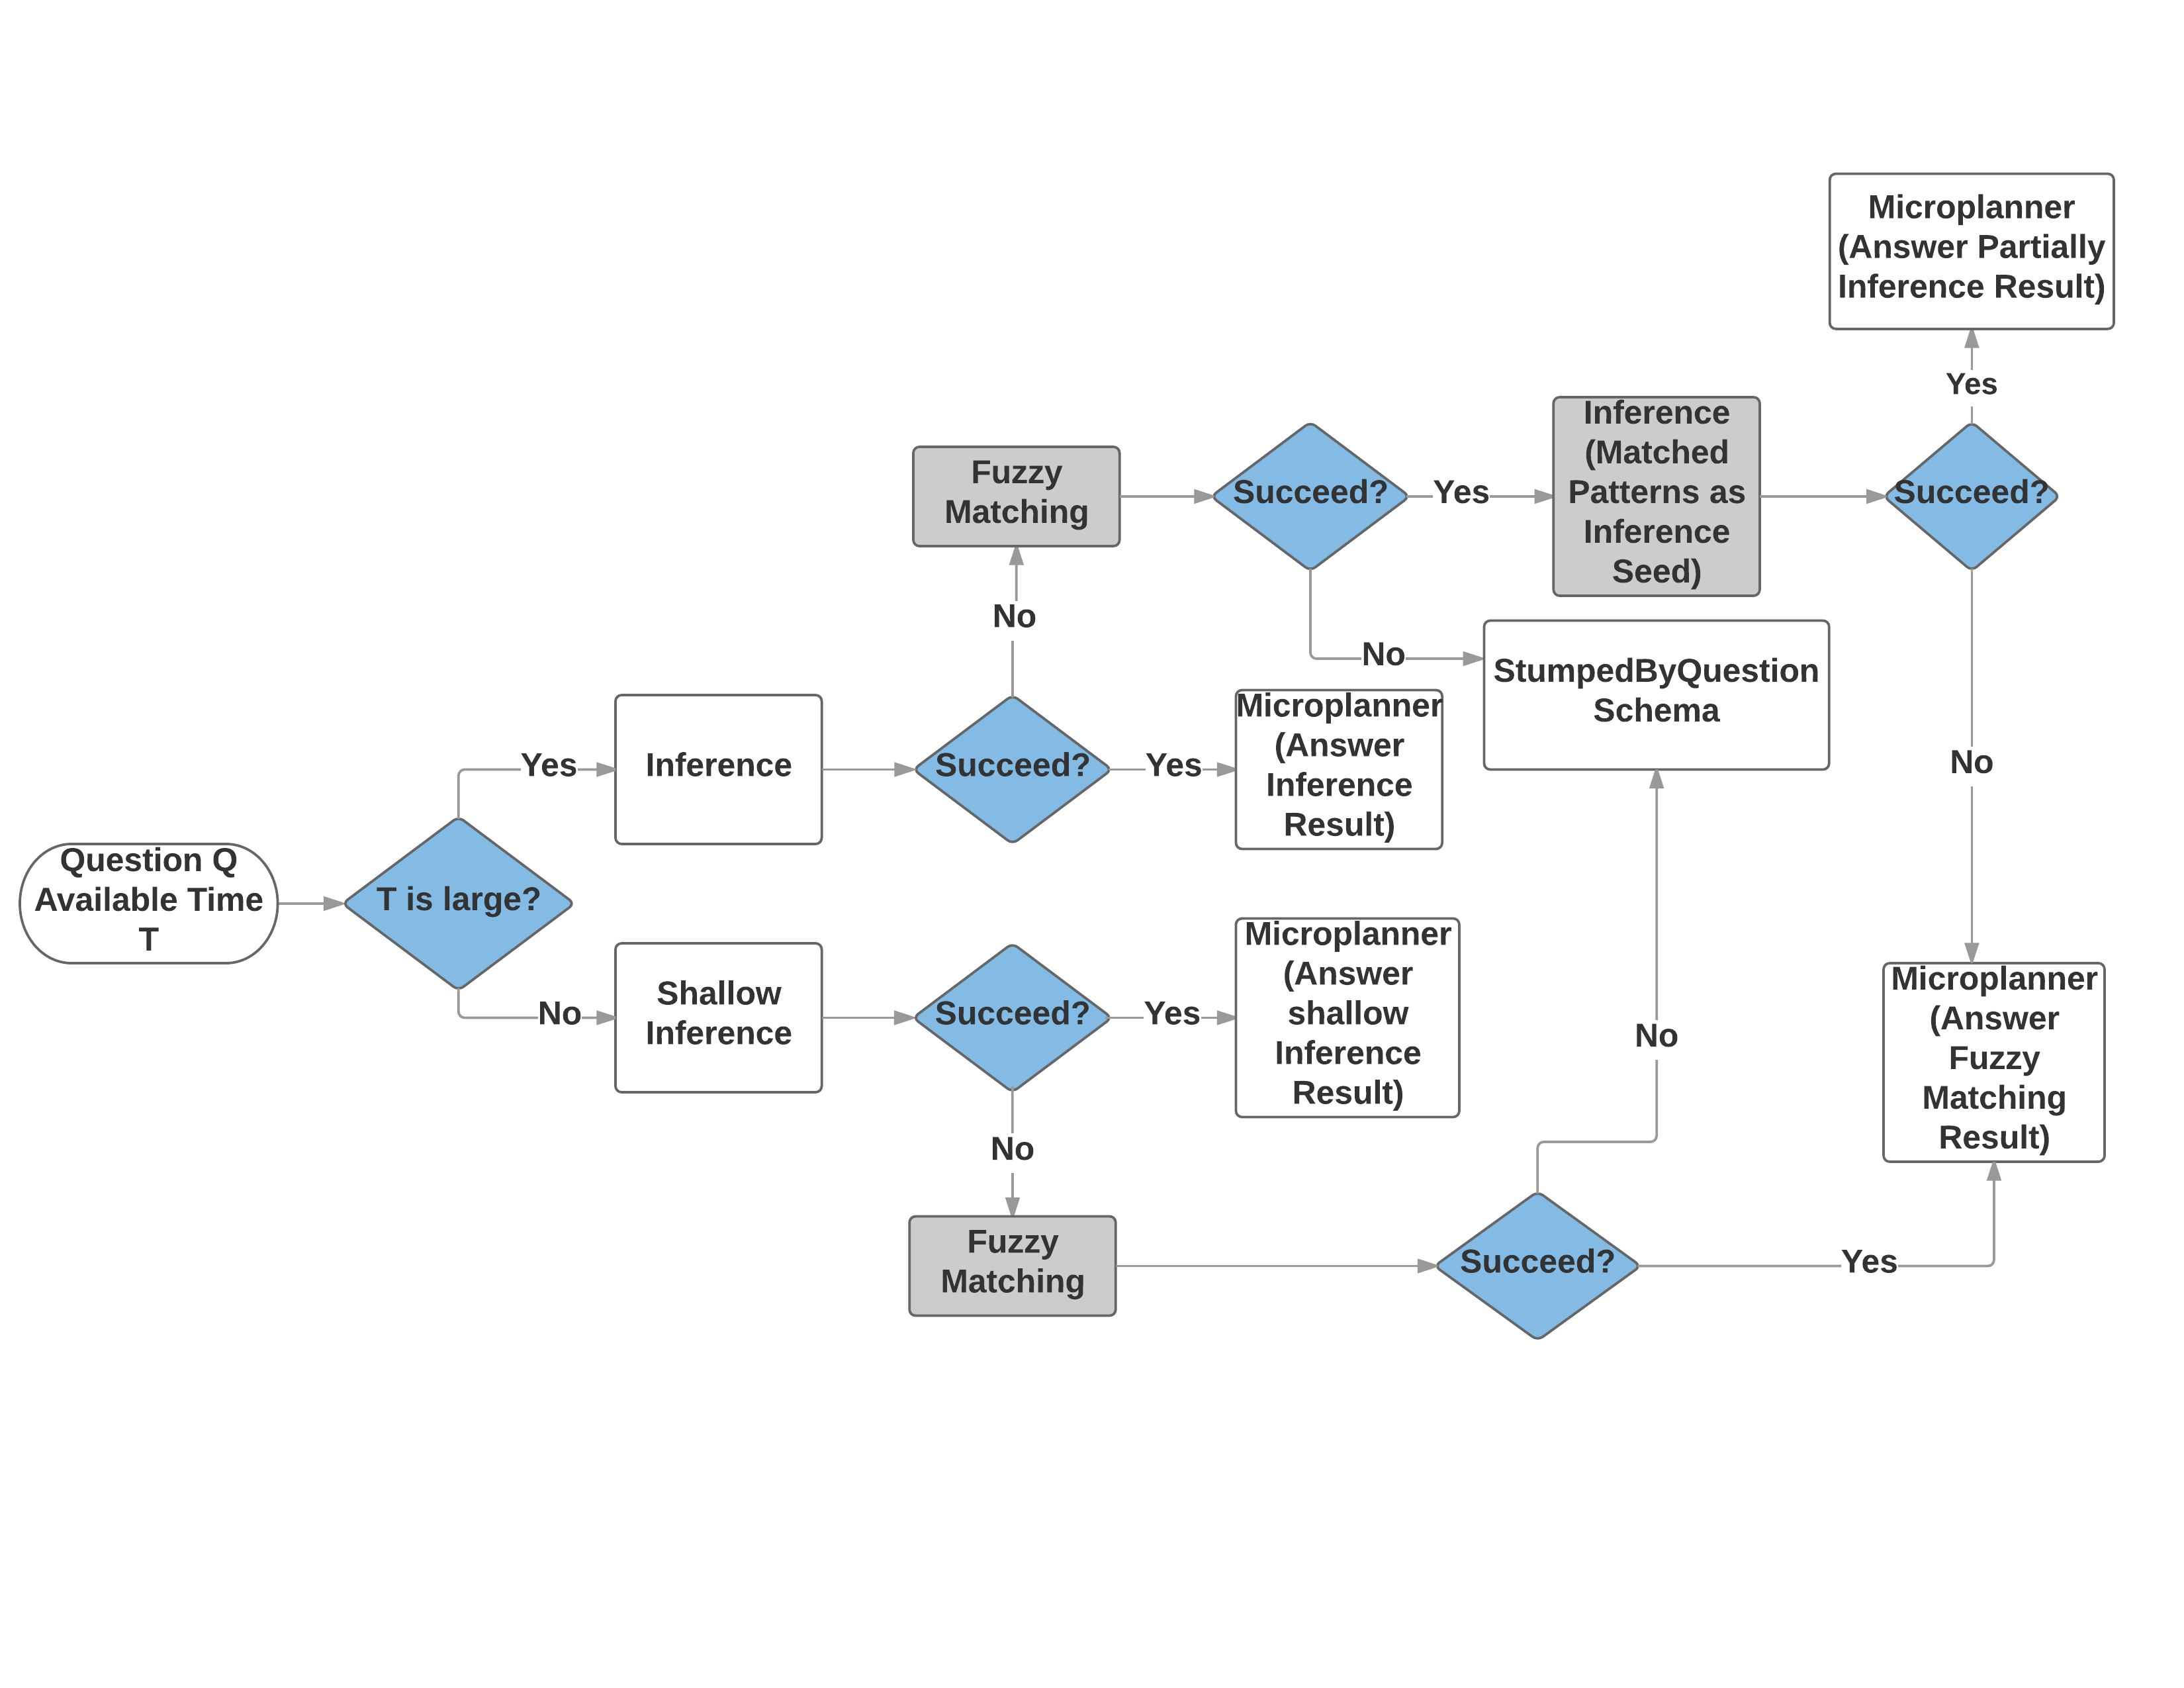
\includegraphics[width=12cm]{figures/QA-schema.png}
\caption{信息查找问答规划器的流程 }
\label{fig:QA-schema}
\end{figure}

其实现方法如下:

\begin{verbatim}
给定一个用于信息查找的问题Q,回答Q的动机,以及所允许的最长等待时间T

如果T的值大,则试图通过逻辑推理来回答Q
     如果成功,则将得到的原子集合输入微观规划器用于应答
     如果失败,则通过基于超图的模糊匹配来回答Q
             如果成功,则将模糊匹配得到的原子集合来做为种子进行进一步推理,试图再次通过逻辑推理来回答Q
                    如果成功,则将得到的原子集合输入微观规划器用于应答
                    如果失败,则将模糊匹配得到的原子集合输入微观规划器用于应答
             如果失败,则触发StumpedByQuestion规划器

如果T的值小,则试图通过浅层推理来快速回答Q
       如果成功,则将得到的原子集合输入微观规划器用于应答
       如果失败,则试图通过基于超图的模糊匹配来回答Q
              如果成功,则将得到的原子集合输入微观规划器用于应答
              如果失败,则触发StumpedByQuestion规划器

\end{verbatim}

\noindent 其中,StumpedByQuestion Schema可规划如下:

\begin{verbatim}
StumpedByQuestion Schema:

给定一个问题Q (其中Q为智能对话系统试图回答但未成功)

当Q的重要值低时,
      触发ExpressIgnorance规划器
				
当Q的重要值很高时,
     使用PLN中的后向链推理找到P,使得
              P ==> Q
     其中,P相对简洁,且上述蕴含推理的真值很高

         如果找到合适的P,将P标记为一个问题,
                并输入到微观规划器用于应答
         如果没有找到合适的P,则
                触发ExpressIgnorance规划器
		

\end{verbatim}

\noindent 其中,ExpressIgnorance规划器可规划如下:

\begin{verbatim}
ExpressIgnorance Schema:

将用于表示"I don't know"  或者
        "I don't know the answer to Q"的原子集合输入微观规划器用于应答
\end{verbatim}

上面例子说明了CogDial方法的本质,我们可以将自适应的语篇管理能力分为下面三个阶段:

\begin{enumerate}
\item 用Scheme或者Python编写相应语篇管理行为代码,然后绑定在GroundedSchemaNodes里。OpenPsi可以在适当的时候调用这些语篇管理行为。
\item 用基于超图的知识表示形式Atom来表示语篇管理行为,通过“硬编码”设置规划器参数,使其调用特定的认知处理程序(如微观规划器Microplanner或者后向链接推理工具Backward Chainer等)。
\item 根据经验,通过强化学习和模仿等方法来自动学习语篇管理行为。
\end{enumerate}

\noindent 很显然,第三种方法是我们最终想要的能进行智能灵活对话的智能会话系统,但也无疑是最难的一种。我们CogDial首先实现第一种方法,然后在此基础上第二和第三种方法。这种增量的开发方式使我们能逐步实现智能的对话处理。使用硬编码的对话管理规划器,能使我们一种很直接的方式不断改进自然语言理解、生成和推理系统中与对话相关的处理,而不是一开始就将这些可能不能处理复杂对话的自然语言处理和推理系统集成到复杂的自动学习对话管理中。当这些模块逐渐完善后,我们将会使用自动学习得到的对话管理规则来替换我们目前使用的手工编写的对话管理规划器。

对于是非(真值查询)问题的应答,可用下面的类似方法来处理:

\begin{verbatim}
Composite Truth-value QA Schema:

给定一个真值查询问题Q,回答该问题的动机,以及所允许的最长等待时间T

试图通过逻辑推理来回答Q
      如果成功,则将得到的原子集合输入微观规划器用于应答
      如果失败,试图通过基于超图的模糊匹配来回答Q
             如果成功,则将模糊匹配得到的原子集合来做为种子进行进一步推理,试图再次通过逻辑推理来回答Q
                    如果成功,则将得到的原子集合输入微观规划器用于应答
                    如果失败,则将模糊匹配得到的原子集合输入微观规划器用于应答
             如果失败,则触发StumpedByQuestion规划器

\end{verbatim}	

\begin{verbatim}
Composite Choice QA Schema:

给定一个选择查询问题Q,供选择的答案C1-Ck,回答该问题的动机,以及所允许的最长等待时机T

重复以下步骤直到T被用完,或者找到一个置信度高的有效答案
       对k个不同的查询“Ci是否为Q的答案”进行并行评估,并对第i个查询赋上其相关的资源r_i
       使用k臂赌博机算法持续重新计算资源分配r_i

如果上述循环返回一个置信度高的有效答案,则将得到的原子集合输入微观规划器用于应答
如果上述循环完成,但没有返回置信度高的有效答案,
       则触发StumpedByQuestion规划器


\end{verbatim}	
			

%%%%%%%%%%%%%%%%%%%%%%%%%%%%%%%%%%%%%%%%%%%%%%%%%%%%%%%%%%%%%%%
\section{实例分析}{Example Dialogues}
%%%%%%%%%%%%%%%%%%%%%%%%%%%%%%%%%%%%%%%%%%%%%%%%%%%%%%%%%%%%%%%
该智能会话系统目前还处于非常初步的阶段,并没有完全实现我们前面章节列出的所有言语规划器和对话控制机制。目前还无法被用做一个很实用的对话系统,但我们认为,在上述的理论分析研究基础上,在完整实现不同的对话控制机制和言语规划器后,CogDial的潜在推理和学习能力能使其成为一个有实用价值的智能会话系统。在本文撰写时,该系统还主要集中在问答机制的实现。本小节给出了一些目前已经实现的简单的对话结果。
\begin{itemize}

\item {\bf CogDial:} Hi there
\begin{itemize}
\item 所使用的言语规划器:开场白(Conventional-Opening)
\end{itemize}

\item {\bf Ruiting:} Hi

\item {\bf CogDial:} What do you want to talk about today?
\begin{itemize}
\item 所使用的言语规划器:开放问题(Open-Question)
\end{itemize}

\item {\bf Ruiting:} What do YOU want to talk about today?

\item {\bf CogDial:} I'm thinking.
\begin{itemize}
\item 所使用的言语规划器:自言自语(Self-talk)
\end{itemize}

\item {\bf Ruiting:} Do people really seek happiness?

\item {\bf CogDial:} Do you seek happiness?
\begin{itemize}
\item 所使用的言语规划器:是非问答(Yes-No Question)
\end{itemize}

\item {\bf Ruiting:} Sometimes...

\item {\bf CogDial:} Hmmm...
\begin{itemize}
\item 所使用的言语规划器:转移话题(Turn-Exit)
\end{itemize}

\item {\bf Ruiting:} Do you have any questions?

\item {\bf CogDial:} I'm tired of asking quesitons.
\begin{itemize}
\item 所使用的言语规划器:是非问答(Yes-No Question)
\end{itemize}
\end{itemize}

%%%%%%%%%%%%%%%%%%%%%%%%%%%%%%%%%%%%%%%%%%%%%%%%%%%%%%%%%%%%%%%
\section{深层语义解析的挑战}{The Challenge of Deep Semantic Understanding for Natural Language}
%%%%%%%%%%%%%%%%%%%%%%%%%%%%%%%%%%%%%%%%%%%%%%%%%%%%%%%%%%%%%%%

在研究和设计智能对话系统中,最具挑战性的并不是上述的复杂推理过程。在给定大知识库Atomspace的情况下,上述的推理过程会变得相当困难,但是我们可以通过在OpenCog中实现的注意力经济分配算法(EConomic Attention AllocatioN, 以下简称ECAN)\cite{Goertzel2010} 来对推理过程进行实时动态规划和控制,虽然ECAN目前仍需进一步的研究和改进,但从我们目前的实验数据来看,该方法是很可行的。在智能对话系统中,比复杂的推理更具有挑战性的问题是,如何使Atomspace获取上述问答规划器中的推理前提的超图表示形式。简单的说,这个挑战也就是如何将自然语言转换成合理准确的语义解析,这恐怕也是实现高度智能化的自然语言对话系统过程中最棘手的问题了。

例如,一个近乎准确的事实“如果A继承Z,那么有很多A在Z的博物馆里”可表示如下:

{\tt\begin{small}\begin{lstlisting}

ImplicationLink <.95,.99>
	ANDLink
		InheritanceLink
			$X
			ConceptNode "museum"
		EvaluationLink
			PredicateNode "of"
			$X
			$Z
	EvaluationLink
		PredicateNode "many"
		SatisfyingSetLink
			ANDLink
				InheritanceLink
					$A
					$Z
				EvaluationLink
					PredicateNode "in"
					$A
					$X

\end{lstlisting}\end{small}}

\noindent 当前的自然语言系统不太可能获取上述例子中想要表达的推理形式。目前的句法分析或语义分析工具也无法根据字典中对博物馆(museum)的解释(如下)来得到上述的推理表达形式。

\begin{verbatim}
museum: a building in which objects of historical, scientific, artistic, or cultural interest are stored and exhibited.
(博物馆:珍藏和陈列历史、科学、艺术或者文化遗产的建筑)
\end{verbatim}

\noindent 但是上述的推理形式可以从自然语言处理系统可以理解的各种句子中推理得出,例如:

\begin{verbatim}
The New York Museum of Modern Art has one of the world's largest collections of French Impressionist works
(纽约的现代艺术博物馆是全球收藏法国印象派作品最多的博物馆之一。)

The British Museum boasts the world's largest Egyptology exhibit, with over five hundred sarcophagi on display,
along with some of the most perfectly preserved examples of engraved hieroglyphics.
(大英博物馆以全球珍藏最多古埃及文物闻名。其中有超过500个石棺,有些还带有保存最完整的象形雕刻文字。)

The US Postal Service Museum hosts enough rare stamps to satisfy even the most avid numismatist, but also
a variety of surprisingly interesting displays recounting, for example, the roles played by various animals in
the history of the postal service.
(美国邮政博物馆拥有足够多的稀有邮票,足以满足即便是最热心的徽章收藏家。不仅如此,该博物馆还展示很多出奇又有趣的历史回放,比如:各种动物扮演的在邮政历史上的不同角色。)

\end{verbatim}

\noindent 通过这些句子提供的信息,得到上述的推理形式就不是特别困难。只需要将这些“大(large)”“足够(enough)”“各种(variety)”等这些量词转换成一般概念层次上的“很多(many)”。而这样的关联完全可以从以下类似的句子中推理得出:

\begin{verbatim}
The New York Museum of Modern Art has one of the world's largest collections of French Impressionist works.
Many of these works are worth tens of millions of dollars, but their artistic value is incalculable.
(纽约的现代艺术博物馆是全球收藏法国印象派作品最多的博物馆之一。
其中很多作品都值上千万美金,但是他们的艺术价值是无价的。)

The dogs had more than enough steaks this morning.  Many of them were rotten but they sure didn't seem to mind.
(狗狗们今天上午吃了太多牛排。其中很多牛排已经馊掉了,但是狗狗似乎一点也不介意。)
\end{verbatim}

\noindent 这些例句能很明确地将其他的量词和“很多(many)”联系起来。例如,解析上面最后一个例句后,RelEx2Logic输出的语义逻辑关系中含有:


 {\tt\begin{small}\begin{lstlisting}
EvaluationLink
	PredicateNode "enough"
	ConceptNode "steaks@5v2"
	
EvaluationLink
	PredicateNode "many"
	ConceptNode "steaks@5v2"
\end{lstlisting}\end{small}}

在解析上面列出的第一个句子后,RelEx2Logic输出的语义逻辑关系中含有:

 {\tt\begin{small}\begin{lstlisting}

 ImplicationLink
 	PredicateNode "largest@737"
	PredicateNode "largest"

EvaluationLink
	PredicateNode "largest@737"
	ConceptNode "collection@a34"
	
EvaluationLink
	PredicateNode "of"
	ConceptNode "collection@a34"
	ConceptNode "works@8fw"
	
EvaluationLink
	PredicateNode "many"
	ConceptNode "works@8fw"
\end{lstlisting}\end{small}}

\noindent 因此如果系统的知识库中含有以下推理常识:

{\tt\begin{small}\begin{lstlisting}
ImplicationLink
	AndLink
		InheritanceLink
			$C
			ConceptNode "collection"
		EvaluationLink
			PredicateNode "of"
			ConceptNode "collection"
			$W
		EvaluationLink
			PredicateNode "many"
			$W
	AndLink
		EvaluationLink
			PredicateNode "many"
			$C
 \end{lstlisting}\end{small}}

\noindent 那么就能推断出:

 {\tt\begin{small}\begin{lstlisting}
ImplicationLink
 	PredicateNode "largest@737"
	PredicateNode "largest"

EvaluationLink
	PredicateNode "largest@737"
	ConceptNode "collection@a34"
	
EvaluationLink
	PredicateNode "many"
	ConceptNode "collection@a34"
\end{lstlisting}\end{small}}

\noindent 如果系统中还有下列常识:

 {\tt\begin{small}\begin{lstlisting}
ImplicationLink
	PredicateNode "largest"
	PredicateNode "large"
\end{lstlisting}\end{small}}

\noindent 那么就能推断出:

 {\tt\begin{small}\begin{lstlisting}
EvaluationLink
	PredicateNode "large"
	ConceptNode "collection@a34"
	
EvaluationLink
	PredicateNode "many"
	ConceptNode "collection@a34"
\end{lstlisting}\end{small}}

Putting these conclusions about enough vs. many and large vs. many, from these sentences, together with similar conclusions from other sentences, the (uncertain) conclusions
将这些从上面例句中推理得来的“大(large)”“足够(enough)”和“很多(many)”相关的结论联合起来,不难得出下列(非确定性)结论:

  {\tt\begin{small}\begin{lstlisting}
ImplicationLink
	EvaluationLink
		PredicateNode "large"
		ConceptNode $X
	EvaluationLink
		PredicateNode "many"
		ConceptNode $X
		
ImplicationLink
	EvaluationLink
		PredicateNode "enough"
		ConceptNode $X
	EvaluationLink
		PredicateNode "many"
		ConceptNode $X
			
\end{lstlisting}\end{small}}

\noindent 这些可以看成是非确定性的启发式的蕴含规则,而这些不确定的直观的知识也正是很多常识性推理的基础。

上述推理中我们假设系统的知识库已存在一定的推理前提,如:

{\tt\begin{small}\begin{lstlisting}
ImplicationLink
	AndLink
		InheritanceLink
			$C
			ConceptNode "collection"
		EvaluationLink
			PredicateNode "of"
			ConceptNode "collection"
			$W
		EvaluationLink
			PredicateNode "many"
			$W
	AndLink
		EvaluationLink
			PredicateNode "many"
			$C
 \end{lstlisting}\end{small}}

\noindent 那么系统如何获取这些假定的直观常识呢,我们的猜想是可以通过自然语言理解系统解析一些相关句子得到,对于本例,系统可以通过解析下面句子获取相关常识:
\begin{verbatim}
His stamp collection is bigger than hers.
(他的邮票收藏库比她的大。)

The bigger bowl has many kinds of candy in it.
(大一点的那个碗里有很多种糖果。)
\end{verbatim}

\noindent 其中第一个句子中的“collection(收藏)”与“bigger(更大)”关联,而第二个句子中“bigger(更大)”与“many(很多)”关联,因此通过演绎推理可以得出“collection(收藏)”与“many(很多)”关联。

\noindent 一般来说,解析某些特定句子所需要的知识都能从其他的句子中获得,但解析这些“其他的句子”可能需要从另外的其他的句子中获取相关知识。因此我们面临的挑战是如何构建一个强大的系统框架,使得获取推理常识的知识网络是一个良性而不是恶性循环。

这个挑战其中一部分是由组合爆炸引起,在我们的超图知识库Atomspace中包括很多不同句子的解析结果,这很容易导致过量的不同推断。上述例子中的任何特定推断理论上都可以通过目标驱动的后向链接推理得出,如\ref{sec:backward}中讨论的回答查询问题的例子“谁在商店买钟琴”中的推理模式,这样一来,我们需要设置Atomspace能储存相对久的知识以保证推理的时候有足够多的推理前提。同样,上述例子中的任何特地推断原则上也可以通过系统自动搜索相关有趣信息来进行前向链接推理得出。不论用哪一种推理方法,不仅需要一个非常丰富复杂的知识库的支持,如果合理高效地进行推理控制更是巨大的研究挑战。

这个挑战并不仅仅是针对查询处理,其实,更关键挑战基本上可以归结为常识推理的问题上\cite{RWR}。考虑到即使是一个简单的常识推理,所涉及的知识领域和其复杂性不言而喻,纯粹通过手工编码构建的复杂知识库如Cyc\cite{Lenat1990}已被证实并不可行。但是随着大数据处理技术的发展,通过分析和挖掘自然语言语料库以及智能体的涉身经验中的语言和非语言信息的综合数据库,来获取常识推理所需要的知识便成为一个更可行有效的方法。然而,根据自然语言的特性,某一个自然语言句子中用于推理的逻辑表现形式,常常与其他句子的表现形式不尽相同,因此通常需要一些从额外的句子中获取的常识来对这些句子进行逻辑形式重排,这也就要求一个可靠的能进行实时不确定逻辑推理系统。这无疑是一个相当棘手的问题。

要解决上述的常识知识问题,对于智能对话系统来说,其中一种方法是粗略模仿人类儿童的语言和认知成长轨迹。也就是说,从相对简单的知识库知识库着手,使得智能对话系统能通过知识库中相对简单的句子和人类交流相对简单的知识。当系统已经建立了基于这些相对简单的知识网络下的常识性知识后,再开始对系统输入稍微复杂的知识--等等,依此下去,这样的对话系统很可能会发展成一个拥有相当的常识语义库并能做出实时合理应答的智能对话系统。

 从概念上讲, 上述方法和\cite{Spitkovsky2013} 中的无监督语言学习类似,即通过逐步将越来越复杂的自然语言句子输入系统,使得系统逐步理解越来越复杂的句子。 \cite{Goertzel2008w} 也提出了类似的涉身行为学习。但我们这里提出的观点更针对智能对话系统,更注重如何从自然语言中抽取出有用的合理的语义知识等的学习。

%%%%%%%%%%%%%%%%%%%%%%%%%%%%%%%%%%%%%%%%%%%%%%%%%%%%%%%%%%%%%%%
\section{本章小结}{Summary of Accomplishments and Future Work}
%%%%%%%%%%%%%%%%%%%%%%%%%%%%%%%%%%%%%%%%%%%%%%%%%%%%%%%%%%%%%%%

目前我们的系统还不足以达到符合人类的智能标准,但这一个介于目前相关研究水平和人类水平之间的对话系统可以看做是使用更可行的研究方法在智能对话系统中集成并完善更多的功能,而不是一味盲目地去追求达到人类水平的目标。

本章充分利用了我们的研究成果,在第\ref{chap:dialogueModel}章中提出的智能会话系统CogDial的概念模型基础上,并结合第\ref{chap:comprehension}章中讨论的自然语言理解系统、第\ref{chap:generation}章中讨论的自然语言生成系统,以及\ref{sec:pln}中讨论的PLN推理系统,以认知模型OpenPsi中的动机机制等技术来设计并实现了几个合理有效的对话管理机制。本章还讨论了我们在智能对话系统的研究中发现的深层语义解析的挑战,也给未来的研究提供了一个明确的方向。下一步工作将进一步完善本章中提出的各种对话管理机制并开发更多新颖智能的对话控制体系结构,并最终运用到机器人或者其他智能体软件系统上。


